\chapter{Tecnologías y Arquitectura de Red}

Una vez establecido el posicionamiento del proyecto respecto del estado del arte, corresponde describir las decisiones tecnológicas concretas que sostienen la implementación del prototipo, así como la arquitectura de red que enmarca su funcionamiento. A diferencia de un desarrollo de software genérico, este proyecto está condicionado por un factor externo determinante: la aplicación no se ejecuta de manera autónoma, sino embebida dentro del panel de administración de Tiendanube, lo que impone restricciones técnicas concretas sobre el lenguaje del frontend y sobre el modo en que la aplicación debe ser servida durante el desarrollo.

\section{Criterios de selección del stack tecnológico}
\label{sec:criterios-seleccion}

Las decisiones tecnológicas del proyecto responden a dos tipos de criterios complementarios. El primero es una restricción impuesta por la plataforma de integración: Tiendanube exige que las aplicaciones integradas a su panel de administración estén construidas sobre React, dado que tanto su \emph{Software Development Kit} (SDK) de comunicación con el panel, \texttt{@tiendanube/nexo} (en adelante, Nexo), como su sistema de diseño oficial, Nimbus, fueron desarrollados específicamente para ese framework. Esta condición no es una preferencia del equipo, sino un requisito no funcional externo que determina de manera directa la tecnología del frontend.

El segundo criterio es una decisión propia del equipo: dado que el frontend debía ser necesariamente JavaScript, se optó por utilizar Node.js también en el backend, de modo de mantener un único lenguaje de programación a lo largo de todo el proyecto. Esta decisión reduce la carga cognitiva de un equipo reducido de dos personas, que debe alternar constantemente entre ambas capas de la aplicación, y evita la duplicación de herramientas de tooling (linters, formateadores, gestores de paquetes) que implicaría sostener dos ecosistemas de lenguajes distintos.

A estos dos criterios se suma una consideración de alcance ya establecida: el proyecto no contempla un despliegue productivo a escala industrial, sino la construcción de un prototipo funcional. Esta definición, presentada en el Alcance del proyecto, habilita decisiones de infraestructura más simples que las que se justificarían en un producto en producción, como se desarrolla en las secciones siguientes.

\section{Organización del código: monorepo}

El proyecto se estructura como un \emph{monorepo}: backend y frontend conviven en un único repositorio, organizados en las carpetas \texttt{backend/} y \texttt{frontend/} respectivamente. Esta decisión responde al fuerte acoplamiento funcional entre ambas capas. Dado que gran parte de los cambios en el proyecto involucra simultáneamente la incorporación o modificación de un endpoint en el backend y su consumo correspondiente en el frontend, un esquema de monorepo permite que ambos cambios se integren en un único commit, evitando que las dos partes queden desincronizadas entre sí, un riesgo real en un esquema de múltiplos repositorios cuando cada uno versiona de forma independiente.

La alternativa de un esquema multi-repo, con versionado y ciclos de despliegue independientes para cada capa, resulta apropiada cuando ambas partes deben evolucionar y desplegarse de forma desacoplada, típicamente en el marco de un despliegue productivo con múltiples equipos. Dado que, como se mencionó, el proyecto no contempla un despliegue productivo a escala industrial sino un prototipo funcional, esa ventaja del multi-repo no aplica en este contexto, mientras que sí se mantiene el costo de coordinación que impone. En consecuencia, el monorepo resulta la opción que mejor equilibra simplicidad operativa y consistencia entre las dos capas de la aplicación.

\section{Stack tecnológico}
\label{sec:stack-tecnologico}

Para cada una de las tecnologías del stack se evaluaron alternativas concretas del ecosistema, con la excepción de React, cuya elección está determinada por un requisito externo ya expuesto en la Sección~\ref{sec:criterios-seleccion}. Estas comparaciones se apoyan en las características técnicas documentadas de cada herramienta y en su adecuación al alcance de un prototipo, y no en pruebas de rendimiento (\emph{benchmarks}) ejecutadas por el equipo; este criterio de evaluación, basado en el análisis de propiedades y no en mediciones propias, es el habitual y académicamente válido para la selección tecnológica de un proyecto de este alcance.

\subsection{Frontend: React, Vite y el ecosistema de Tiendanube}
\label{sec:frontend-react-vite}

El frontend está desarrollado en React (versión \texttt{19.2.7}), servido mediante Vite (versión \texttt{8.1.1}) como herramienta de \emph{build} y servidor de desarrollo. Como se indicó, la elección de React no es opcional: Tiendanube exige este framework para las aplicaciones integradas a su panel de administración, dado que su SDK Nexo y su sistema de diseño Nimbus están construidos específicamente para él. Nexo es responsable de establecer la comunicación entre la aplicación, ejecutada dentro de un \emph{iframe}, y la ventana del panel de administración que la contiene, mientras que Nimbus provee los componentes visuales con los que la interfaz del prototipo mantiene consistencia estética con el resto del panel de Tiendanube, cuyo uso Tiendanube exige explícitamente en sus aplicaciones integradas como condición de calidad y consistencia \parencite{TiendanubeAPI2024}.

Sobre esa base obligatoria de React, Vite fue seleccionado como herramienta de desarrollo por sus características propias: a diferencia de herramientas de \emph{build} más antiguas, Vite sirve el código fuente mediante módulos ES nativos del navegador durante el desarrollo, lo que se traduce en un servidor de arranque prácticamente instantáneo y en actualización en caliente (\emph{Hot Module Replacement}) de los cambios, agilizando el ciclo de desarrollo iterativo propio de un prototipo.

Si bien React fue impuesto por Tiendanube, la herramienta de \emph{build} no lo estaba: sobre esa decisión sí se evaluaron alternativas. La Tabla~\ref{tab:comparativo_bundler} resume la comparación realizada entre Vite, Create React App y Next.js.

Vite se consolidó como la opción elegida por ser el estándar actual para proyectos de React de tipo SPA. Create React App se descartó por encontrarse discontinuado, y Next.js por aportar capacidades ---renderizado del lado del servidor y un sistema de enrutado propio--- que carecen de sentido en una aplicación que se renderiza embebida dentro del \emph{iframe} del panel de administración de Tiendanube.

La integración entre Vite, Nexo y el entorno de túneles necesario para el desarrollo (descripto en la Sección~\ref{sec:arquitectura-red}) no resultó automática. Nexo fue diseñado originalmente para entornos Node.js y referencia en su código la variable global \texttt{global}, inexistente en el navegador; sin una configuración adicional, la aplicación fallaba al iniciar con el error \texttt{Uncaught ReferenceError: global is not defined}, que se traducía en una pantalla en blanco dentro del \emph{iframe}. La solución consistió en instruir a Vite, mediante la opción \texttt{define: \{ global: 'globalThis' \}}, para reemplazar en el código empaquetado todas las referencias a \texttt{global} por \texttt{globalThis}, sí disponible en los navegadores modernos. De manera similar, Vite bloquea por defecto las peticiones entrantes desde hosts externos al del propio servidor de desarrollo, lo cual entra en conflicto directo con el uso de un túnel público (Sección~\ref{sec:arquitectura-red}): al acceder a la aplicación mediante su URL pública, el navegador recibía el error \texttt{Blocked request. This host is not allowed}. Esto se resolvió habilitando explícitamente el dominio del proveedor de túnel en \texttt{server.allowedHosts}. Ambos ajustes ilustran que, más allá de la elección del framework y la herramienta de \emph{build}, buena parte del trabajo técnico consistió en conciliar un SDK pensado para Node.js con las restricciones propias del navegador y de la arquitectura de red descripta más adelante.

\begin{table}[h]
\centering
\caption{Comparación de herramientas de \emph{build} para el frontend en React}
\label{tab:comparativo_bundler}
\renewcommand{\arraystretch}{1.3}
\begin{tabular}{|m{2.3cm}|m{4.4cm}|m{4.4cm}|m{3.4cm}|}
\hline
\textbf{Opción} & \textbf{Ventajas} & \textbf{Consideraciones} & \textbf{Decisión} \\
\hline
Vite & Estándar moderno para \emph{Single Page Applications} (SPA) de React; arranque y actualización en caliente muy rápidos; liviano; configuración simple & --- & \textbf{Elegido.} Apropiado para una SPA de React que se embebe en un \emph{iframe} \\
\hline
Create React App & Fue el estándar histórico para proyectos de React & Obsoleto y sin mantenimiento activo; más lento & Descartado por tratarse de una herramienta discontinuada \\
\hline
Next.js & Framework full-stack; renderizado del lado del servidor (SSR); enrutado propio & El SSR y el enrutado propio resultan innecesarios para una SPA embebida en un \emph{iframe}; sobredimensionado para el caso de uso & Descartado: sus capacidades no aplican a una aplicación que corre dentro del panel de Tiendanube \\
\hline
\end{tabular}
\end{table}

\subsection{Backend: Node.js y Express}
\label{sec:backend-node-express}

El backend está desarrollado en Node.js, en su versión 18 o superior, único requisito de versión documentado para el proyecto, utilizando Express como framework para la construcción de la API REST. Como se explicó en la Sección~\ref{sec:criterios-seleccion}, la elección de Node.js responde directamente a la necesidad de mantener un único lenguaje de programación en todo el proyecto, una vez que el frontend quedó determinado por el requisito de React de Tiendanube. Express fue seleccionado por tratarse de un framework minimalista y no dogmático, ampliamente adoptado para la construcción de API REST, que permite definir rutas y middlewares con una curva de aprendizaje reducida, adecuada al alcance de un prototipo desarrollado por un equipo de dos personas.

Esta elección tampoco fue arbitraria: se evaluaron las principales alternativas del ecosistema Node.js antes de decidir. La Tabla~\ref{tab:comparativo_backend} resume la comparación.

El criterio que definió la elección fue el tamaño del ecosistema y la documentación disponible, junto con el hecho de que Express no impone una estructura particular al proyecto. El rendimiento no constituyó un factor determinante, dado que no representaba una preocupación para un prototipo, y la arquitectura más robusta de NestJS se descartó por introducir una complejidad que no se traducía en un beneficio concreto para el alcance definido.

El backend cumple dos funciones centrales. Por un lado, actúa como intermediario autenticado entre el frontend y la API de Tiendanube: es quien retiene las credenciales de la aplicación (\texttt{Client ID} y \texttt{Client Secret}) y ejecuta el intercambio OAuth 2.0 descripto en la Sección~\ref{sec:estrategia-datos-ref}, de modo que dichas credenciales nunca se exponen al frontend ni al \emph{iframe} embebido en el navegador del usuario. Por otro lado, expone los \emph{webhooks} de privacidad que Tiendanube exige a toda aplicación integrada a su ecosistema (\texttt{/api/webhooks/store-redact}, \texttt{customers-redact} y \texttt{customers-data-request}), mediante los cuales la plataforma notifica solicitudes de eliminación de datos en cumplimiento de normativas de protección de datos personales.

\begin{table}[h]
\centering
\caption{Comparación de frameworks de backend para Node.js}
\label{tab:comparativo_backend}
\renewcommand{\arraystretch}{1.3}
\begin{tabular}{|m{2.3cm}|m{4.4cm}|m{4.4cm}|m{3.4cm}|}
\hline
\textbf{Framework} & \textbf{Ventajas} & \textbf{Desventajas} & \textbf{Decisión} \\
\hline
Express & Ecosistema y documentación más amplios dentro de Node.js; minimalista; no impone una estructura; gran cantidad de ejemplos y soluciones disponibles & Menos funcionalidades incluidas por defecto que NestJS; rendimiento algo menor que Fastify & \textbf{Elegido.} La opción más simple y documentada para una API REST de prototipo \\
\hline
Fastify & Mayor rendimiento; validación de esquemas integrada & Ecosistema más reducido; su principal ventaja (velocidad) no constituía una necesidad del proyecto & Descartado: la performance adicional no aportaba valor a un prototipo \\
\hline
NestJS & Arquitectura robusta; adecuado para aplicaciones grandes y equipos numerosos & Estructura opinada y pesada; mayor curva de aprendizaje; sobredimensionado para el alcance del proyecto & Descartado por complejidad innecesaria para el tamaño del proyecto \\
\hline
Koa & Diseño moderno; manejo de middleware más limpio & Ecosistema y comunidad más pequeños; menos material de referencia disponible & Descartado: menor soporte que Express sin una ventaja decisiva \\
\hline
\end{tabular}
\end{table}

\subsection{Persistencia: PostgreSQL}

Para la capa de persistencia se seleccionó PostgreSQL como motor de base de datos relacional. La base de datos fue incorporada al proyecto para la presente entrega: el prototipo persiste en PostgreSQL tanto los datos obtenidos de la tienda de desarrollo a través de la API de Tiendanube como el conjunto de datos generado mediante el script de generación aleatoria controlada descripto en la Sección 2.6, siguiendo el modelo de datos presentado en la Figura~\ref{fig:erd-diagram}. El esquema implementado replica las entidades documentadas en el Marco Teórico (tiendas, productos, variantes, clientes y pedidos), preservando las relaciones e integridad referencial entre ellas.

Antes de definir el motor específico, se evaluó el enfoque relacional frente al no relacional. Se optó por un modelo relacional porque los datos del dominio son inherentemente relacionales: los pedidos se componen de ítems que referencian variantes, las cuales pertenecen a su vez a productos, y los clientes se vinculan a sus pedidos, tal como se describió al detallar los recursos consumidos de la API de Tiendanube en el Marco Teórico. Estas relaciones, que requieren integridad referencial, se modelan de forma natural en un motor relacional, tal como reflejará el diagrama de base de datos del proyecto. La Tabla~\ref{tab:comparativo_db_enfoque} resume esta primera comparación.

Una vez definido el enfoque relacional, se compararon los motores disponibles. La Tabla~\ref{tab:comparativo_db_motor} resume la comparación entre PostgreSQL, MySQL y SQLite.

Conviene precisar que PostgreSQL y MySQL resultaban ambos válidos para el proyecto: la elección del primero no responde a una deficiencia del segundo, sino a su soporte de tipos JSONB y a ser el estándar más habitual en el stack de Node.js moderno.

El acceso a la base de datos se implementa mediante Prisma como \emph{Object-Relational Mapping} (ORM). Esta elección responde a los mismos criterios que guiaron la selección del resto del stack (Sección~\ref{sec:criterios-seleccion}): al tratarse de un equipo reducido de dos personas, Prisma permite definir el esquema de datos de forma declarativa en un único archivo, generar automáticamente un cliente tipado en JavaScript y gestionar las migraciones de forma reproducible, evitando la escritura manual de SQL y la duplicación de herramientas entre las capas del proyecto. El esquema de Prisma refleja directamente el modelo de datos presentado en la Figura~\ref{fig:erd-diagram}.

\begin{figure}[ht]
    \centering
    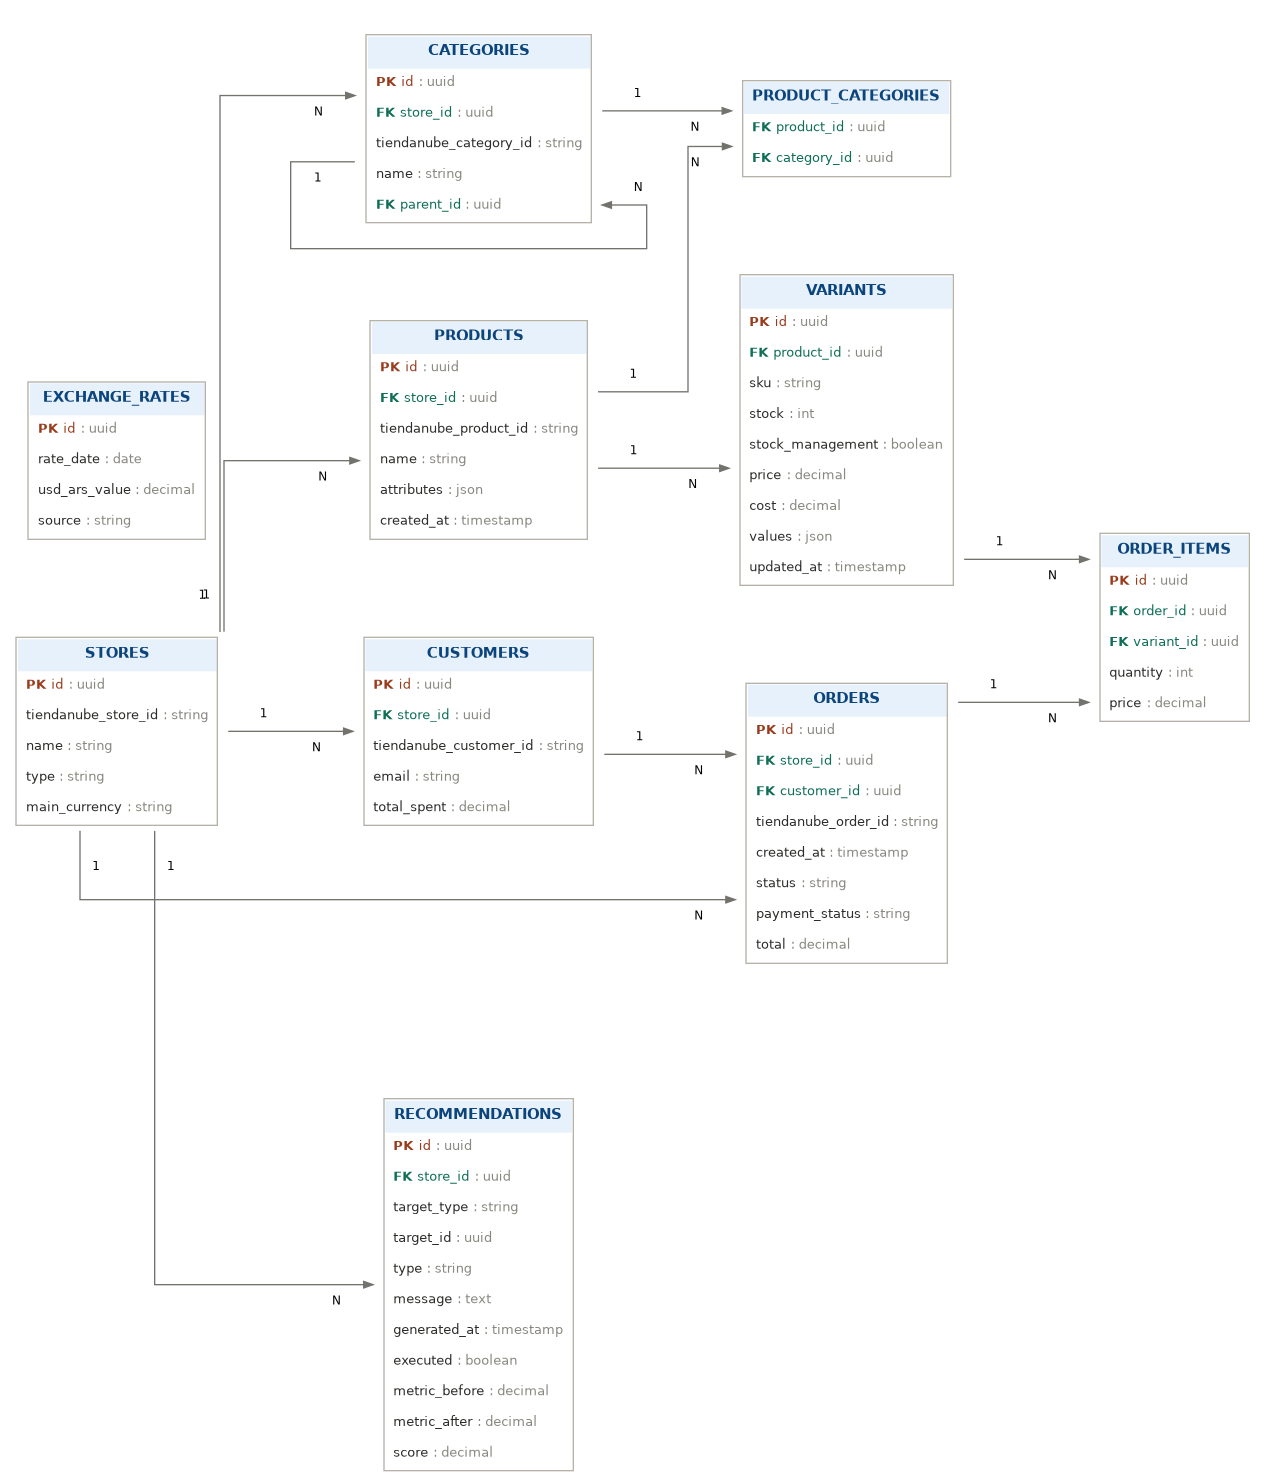
\includegraphics[width=\textwidth]{./images/erd_diagram.png}
    \caption{Diagrama entidad-relación (ERD) del modelo de datos del prototipo.}
    \label{fig:erd-diagram}
\end{figure}

\noindent\textit{Fuente: elaboración propia.}

El esquema se organiza en torno a \texttt{STORES} como entidad raíz de aislamiento multi-tienda: la clave foránea \texttt{store\_id} se repite en \texttt{CATEGORIES}, \texttt{PRODUCTS}, \texttt{CUSTOMERS}, \texttt{ORDERS} y \texttt{RECOMMENDATIONS}, garantizando que los datos de cada comercio conectado permanezcan separados entre sí. Sobre esa base, \texttt{PRODUCTS} se vincula con \texttt{VARIANTS} en una relación uno a muchos, reflejando la distinción entre un producto y sus combinaciones concretas de talle, color u otro atributo descripta en la Sección~\ref{sec:adquisicion-datos} del Marco Teórico, mientras que \texttt{CATEGORIES} se relaciona con \texttt{PRODUCTS} a través de la tabla intermedia \texttt{PRODUCT\_CATEGORIES} y admite una jerarquía propia mediante \texttt{parent\_id}, lo que permite segmentar las recomendaciones por rubro comercial tal como se planteó en la Sección~\ref{sec:comportamiento-consumidor}. Los pedidos, por su parte, se modelan mediante \texttt{ORDERS} y su detalle \texttt{ORDER\_ITEMS}, que referencia cada variante junto con la cantidad y el precio de la operación, y \texttt{CUSTOMERS} conserva el campo \texttt{total\_spent} provisto directamente por la API de Tiendanube y descripto en esa misma sección.

Dos entidades del esquema no se limitan a replicar recursos de la API de Tiendanube, sino que materializan capacidades propias del prototipo. \texttt{RECOMMENDATIONS} implementa el mecanismo de retroalimentación presentado en la Sección~\ref{sec:feedback-loop} del Marco Teórico: el campo \texttt{executed} registra si el comerciante llevó a cabo la acción sugerida, \texttt{metric\_before} y \texttt{metric\_after} sostienen la comparación de impacto entre ventanas temporales, y \texttt{score} persiste la priorización dinámica que ese mecanismo actualiza en función de los resultados obtenidos. \texttt{EXCHANGE\_RATES}, por su parte, almacena el valor diario del dólar oficial y del dólar blue consultado ante la API pública de tipo de cambio mencionada en el Alcance del proyecto, dato de contexto auxiliar que las recomendaciones del rubro electrónica utilizan para detectar la desactualización de precios frente a movimientos cambiarios, según se caracterizó en la Sección~\ref{sec:comportamiento-consumidor}.

\FloatBarrier

\begin{table}[h]
\centering
\caption{Comparación entre modelo de datos relacional y no relacional}
\label{tab:comparativo_db_enfoque}
\renewcommand{\arraystretch}{1.3}
\begin{tabular}{|m{2.3cm}|m{4.4cm}|m{4.4cm}|m{3.4cm}|}
\hline
\textbf{Enfoque} & \textbf{Ventajas} & \textbf{Consideraciones} & \textbf{Decisión} \\
\hline
Relacional & Modela relaciones con integridad referencial; adecuado para datos estructurados y vinculados entre sí (pedidos, productos y clientes) & Esquema más rígido & \textbf{Elegido.} Los datos del dominio son relacionales por naturaleza \\
\hline
No relacional (MongoDB) & Flexible para datos no estructurados; permite escalado horizontal & Débil para relaciones complejas; sin integridad referencial nativa & Descartado: los datos del dominio requieren relaciones, no flexibilidad de esquema \\
\hline
\end{tabular}
\end{table}

\subsection{Túnel de desarrollo: ngrok}
\label{sec:tunel-ngrok}

El uso de ngrok como herramienta de túnel HTTPS es una consecuencia directa de la arquitectura de integración con Tiendanube, y se desarrolla en detalle en la Sección~\ref{sec:arquitectura-red}. Cabe adelantar que su necesidad no es una elección arbitraria de infraestructura, sino la solución a una restricción concreta: Tiendanube no admite que una aplicación de prueba se sirva desde una URL \texttt{localhost}, y requiere en su lugar una URL pública con HTTPS. ngrok resuelve esta necesidad generando, a partir del servidor de desarrollo local, una URL pública que actúa como túnel hacia dicho servidor, sin requerir desplegar la aplicación en un servidor propio durante la etapa de desarrollo.

Esta elección se comparó puntualmente frente a Vercel, plataforma ya conocida por el equipo. Ambas herramientas, sin embargo, resuelven problemas distintos: ngrok es un túnel de desarrollo que expone un entorno local ya en ejecución, mientras que Vercel es una plataforma de despliegue que publica una aplicación empaquetada. La Tabla~\ref{tab:comparativo_tunel} resume esta comparación.

Lo que definió la elección fue que ngrok resuelve la necesidad concreta de exponer el entorno local sin implicar un despliegue productivo, explícitamente fuera del alcance del proyecto según lo establecido en el Alcance. La limitación inicial de la URL cambiante entre sesiones, propia del uso por defecto del plan gratuito, se resolvió mediante el dominio fijo gratuito que ngrok ofrece, lo cual elimina la necesidad de reconfigurar manualmente la URL en la sección ``Aplicación de Prueba'' del panel de Partners de Tiendanube en cada reinicio del túnel. Vercel no queda descartado de forma definitiva: al no ser una alternativa peor sino una herramienta con otro propósito, se mantiene como opción a reevaluar para publicar la aplicación terminada de cara a la defensa del proyecto.

\begin{table}[h]
\centering
\caption{Comparación entre motores de base de datos relacionales}
\label{tab:comparativo_db_motor}
\renewcommand{\arraystretch}{1.3}
\begin{tabular}{|m{2.3cm}|m{4.4cm}|m{4.4cm}|m{3.4cm}|}
\hline
\textbf{Motor} & \textbf{Ventajas} & \textbf{Consideraciones} & \textbf{Decisión} \\
\hline
PostgreSQL & Soporte robusto de JSONB, útil para almacenar respuestas de la API con estructura flexible; estándar habitual en el stack de Node.js moderno; de código abierto y gratuito & Configuración algo más pesada que SQLite & \textbf{Elegido} por su soporte de JSONB y por ser el estándar más común del stack \\
\hline
MySQL & Muy difundido; buen rendimiento; también gratuito & Soporte de JSON algo menos potente que el JSONB de PostgreSQL & Alternativa igualmente válida; la elección se inclinó por PostgreSQL, no por una deficiencia de MySQL \\
\hline
SQLite & Configuración nula; adecuado para prototipos muy pequeños & No apto para concurrencia; limitado para escalar & Considerado únicamente como opción de arranque inicial \\
\hline
\end{tabular}
\end{table}

\begin{table}[h]
\centering
\caption{Comparación entre ngrok y Vercel para exponer el entorno de desarrollo}
\label{tab:comparativo_tunel}
\renewcommand{\arraystretch}{1.3}
\begin{tabular}{|m{2.3cm}|m{4.4cm}|m{4.4cm}|m{3.4cm}|}
\hline
\textbf{Opción} & \textbf{Rol / Ventajas} & \textbf{Consideraciones} & \textbf{Decisión} \\
\hline
ngrok & Túnel de desarrollo: expone el entorno local al \emph{iframe} de Tiendanube de forma instantánea, preservando la actualización en caliente; dominio fijo disponible en su plan gratuito & La URL pública cambiaba entre sesiones bajo el uso por defecto del plan gratuito & \textbf{Elegido} para el entorno de desarrollo: resuelve exactamente la necesidad de exponer el entorno local \\
\hline
Vercel & Plataforma de despliegue: publica la aplicación en una URL pública y estable & Es una herramienta de \emph{deployment}, no un túnel de desarrollo; un backend Express tradicional requiere adaptación a su modelo \emph{serverless}; desplegar implica un despliegue productivo, fuera del alcance del proyecto & No aplicable al desarrollo; se reevalúa como opción para publicar la aplicación terminada de cara a la defensa \\
\hline
\end{tabular}
\end{table}

\section{Arquitectura de red}
\label{sec:arquitectura-red}

La arquitectura de red del prototipo está determinada por el hecho de que la aplicación no se accede de forma directa, sino que se embebe como un \emph{iframe} dentro del panel de administración de Tiendanube, servido este último desde los servidores de la plataforma bajo HTTPS. Los navegadores modernos bloquean por política de \emph{contenido mixto} la carga de un \emph{iframe} servido por HTTP dentro de una página servida por HTTPS; en consecuencia, la aplicación embebida debe estar disponible también bajo una URL pública con HTTPS, incluso durante el desarrollo, donde de otro modo bastaría con \texttt{localhost}. Esta restricción es la que motiva el uso de ngrok, introducido en la sección anterior.

La Figura~\ref{fig:arquitectura-red} sintetiza el flujo completo de comunicación en el entorno de desarrollo, detallado a continuación paso a paso.

\begin{figure}[ht]
    \centering
    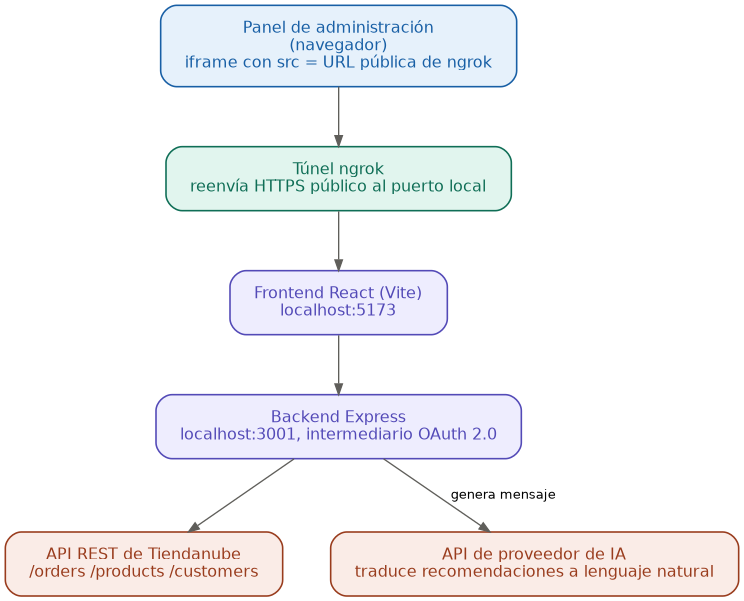
\includegraphics[width=\textwidth]{./images/diagrama_arquitectura_red.png}
    \caption{Arquitectura de red del prototipo en el entorno de desarrollo.}
    \label{fig:arquitectura-red}
\end{figure}

\vspace{6pt}
\noindent\textit{Fuente: elaboración propia.}

El flujo completo de comunicación, en el entorno de desarrollo, puede describirse en los siguientes pasos:

\begin{enumerate}
    \item Dentro del panel de administración de la tienda (servido por Tiendanube), el comerciante accede a la sección correspondiente a la aplicación, que Tiendanube renderiza como un \emph{iframe} cuyo origen (\texttt{src}) es la URL pública HTTPS provista por ngrok.

    \item ngrok reenvía el tráfico recibido en esa URL pública hacia el servidor de desarrollo de Vite, expuesto localmente en el puerto 5173, que sirve el frontend de React.

    \item Una vez cargado dentro del \emph{iframe}, el frontend inicializa el SDK Nexo, que establece comunicación con la ventana del panel de administración (la ventana padre) para obtener el contexto de la tienda y habilitar la sesión de la aplicación para ese comercio en particular.

    \item El frontend, aunque accedido a través de la URL pública de ngrok, se ejecuta en el navegador de la misma máquina donde corre el entorno de desarrollo. Por lo tanto, sus llamadas a la API propia de la aplicación se realizan directamente contra el backend en \texttt{localhost:3001}, sin necesidad de atravesar el túnel de ngrok.

    \item El backend, sobre la base del token obtenido mediante el flujo OAuth 2.0 descripto en la Sección~\ref{sec:estrategia-datos-ref} del Marco Teórico, consume los recursos correspondientes de la API REST de Tiendanube (\texttt{/orders}, \texttt{/products}, \texttt{/customers}, entre otros, detallados en esa misma sección) \parencite{TiendanubeAPI2024}, y devuelve al frontend los datos ya procesados.

    \item El frontend renderiza la respuesta dentro del \emph{iframe}, integrada visualmente al panel de administración mediante los componentes de Nimbus.
\end{enumerate}

Esta topología de red es propia del entorno de desarrollo y depende de un túnel de terceros (ngrok) en lugar de una infraestructura de \emph{hosting} propia. Tal como se detalla en la Sección~\ref{sec:tunel-ngrok}, esta elección fue evaluada frente a una plataforma de despliegue (Vercel) y resulta adecuada mientras el despliegue productivo permanezca fuera del alcance del prototipo; una eventual publicación formal en la tienda de aplicaciones de Tiendanube, señalada como trabajo futuro en el Alcance del proyecto, sí requeriría reemplazar este túnel por una solución de \emph{hosting} permanente.

A la fecha de esta entrega, esta arquitectura fue validada de manera funcional de extremo a extremo: la aplicación carga correctamente embebida dentro del \emph{iframe} del panel de administración de la tienda de desarrollo de Tiendanube, con el intercambio (\emph{handshake}) de Nexo funcionando de forma correcta entre el \emph{iframe} y la ventana padre.

\section{Entorno de desarrollo}

Levantar el entorno de desarrollo completo requiere ejecutar tres procesos en simultáneo: el backend (\texttt{cd backend \&\& npm run dev}, puerto 3001), el frontend (\texttt{cd frontend \&\& npm run dev}, puerto 5173) y el túnel de ngrok (\texttt{ngrok http 5173}). Esta separación en tres procesos independientes refleja directamente la arquitectura de red descripta en la Sección~\ref{sec:arquitectura-red}: cada uno de ellos corresponde a un componente distinto del flujo de comunicación (servidor de API, servidor de la interfaz y túnel público).

La configuración de cada capa se administra mediante variables de entorno independientes en cada carpeta del monorepo. El backend concentra las credenciales sensibles de la aplicación (\texttt{Client ID} y \texttt{Client Secret} de Tiendanube), mientras que el frontend recibe únicamente el \texttt{Client ID}, dato público necesario para inicializar el SDK Nexo del lado del navegador. Esta separación no es incidental: mantiene el \texttt{Client Secret} fuera del código que se ejecuta en el navegador del usuario, en línea con el rol del backend como intermediario autenticado descripto en la Sección~\ref{sec:backend-node-express}. Cabe señalar, además, que Vite solo lee las variables de entorno del frontend al iniciar el proceso, por lo que una modificación en su archivo de configuración requiere reiniciar el servidor de desarrollo correspondiente para que los nuevos valores se apliquen.
